
\documentclass{article}
\usepackage{tikz}
\usetikzlibrary{arrows,shapes,trees}

\begin{document}
\section{Magic School Evolution}
\begin{center}
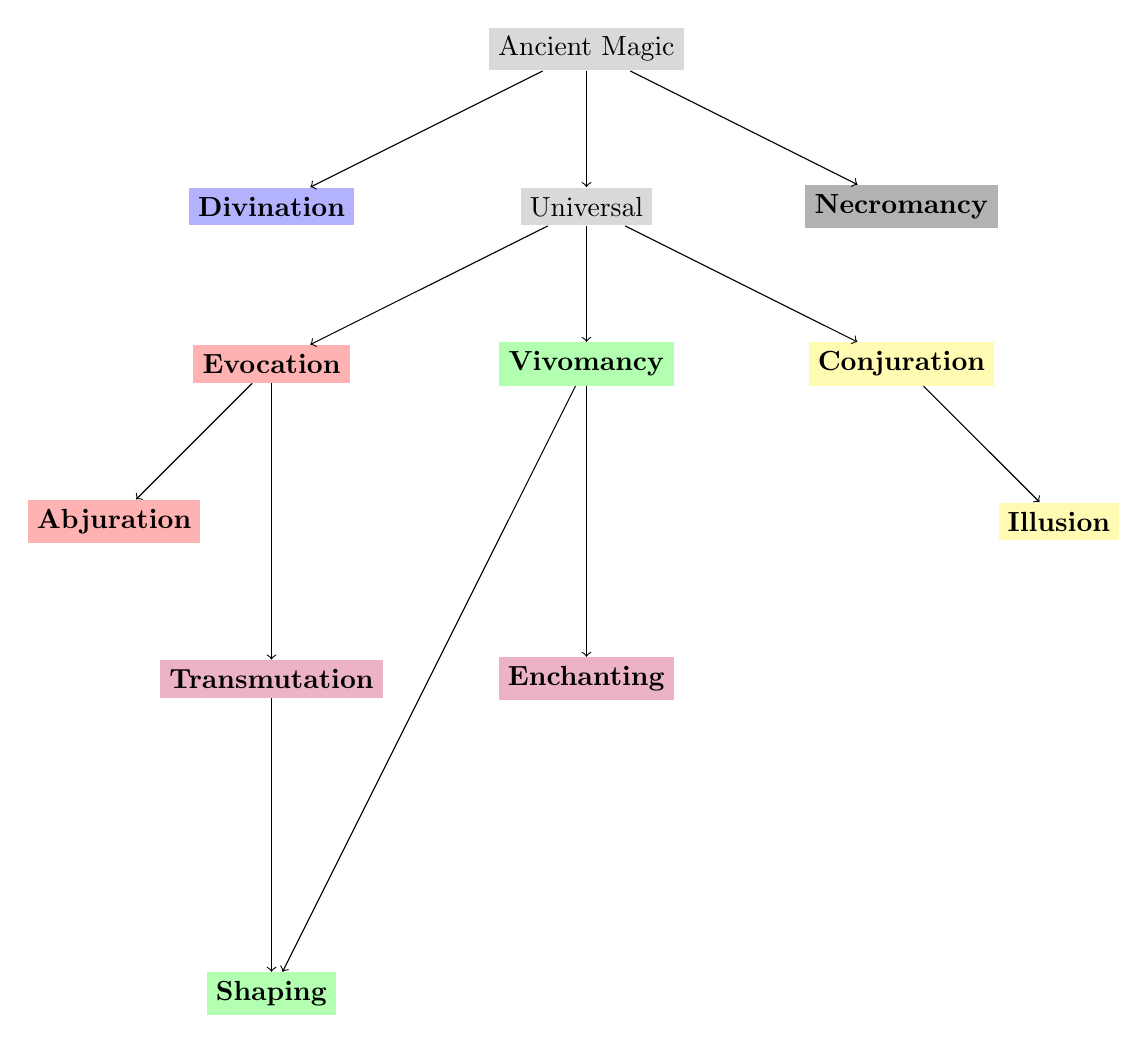
\begin{tikzpicture}[scale=2.0]
\tikzstyle{every node} = [rectangle]
\node[fill=gray!30] (root) at (3, 6) {Ancient Magic};
\node[fill=blue!30] (divination) at (1,5) {\textbf{Divination}};
\node[fill=gray!30] (univ) at (3,5) {Universal};
\node[fill=red!30] (evoc) at (1, 4) {\textbf{Evocation}};
\node[fill=green!30] (vivo) at (3, 4) {\textbf{Vivomancy}};
\node[fill=yellow!30] (conjur) at (5, 4) {\textbf{Conjuration}};
\node[fill=red!30] (abjur) at (0, 3) {\textbf{Abjuration}};
\node[fill=yellow!30] (illusion) at (6, 3) {\textbf{Illusion}};
\node[fill=black!30] (necro) at (5, 5) {\textbf{Necromancy}};
\node[fill=purple!30] (enchant) at (3, 2) {\textbf{Enchanting}};
\node[fill=purple!30] (transmute) at (1,2) {\textbf{Transmutation}};
\node[fill=green!30] (shapers) at (1,0) {\textbf{Shaping}};

\draw [->] (root) -- (divination);
\draw [->] (root) -- (univ);
\draw [->] (root) -- (necro);
\draw [->] (univ) -- (evoc);
\draw [->] (univ) -- (vivo);
\draw [->] (univ) -- (conjur);
\draw [->] (evoc) -- (abjur);
\draw [->] (conjur) -- (illusion);
\draw [->] (evoc) -- (transmute);
\draw [->] (vivo) -- (enchant);
\draw [->] (transmute) -- (shapers);
\draw [->] (vivo) -- (shapers);
\end{tikzpicture}
\end{center}

\section{Magic Schools}
\subsection{Abjuration}
Abjuration is a school focused on using magical energy for defense of the spellcaster or the target of the spell. It was an early offshoot of evocation, developed in response to evokers looking at methods of protecting themselves from their own spells.

\subsection{Conjuration}
Conjuration is a school focused on using magic to call, summon, or create things. The earliest form of conjuration focused on calling creatures to the caster. Later forms delved into extra-dimensional summoning and gating.
Call Beast, Dimensional Door, and Gate are all conjuration spells.

\subsection{Divination}
Divination is a school focused on the gathering of knowledge. The oldest school known, divination first appeared while humans were still in the tribal phase. Shamans and witch-doctors would cast spells to gather knowledge to help them bring their tribes to victory. Despite being the oldest known school of magic officially studied, Diviners are quiet often dismissed as being relatively powerless. This attitude eventually lead to the split in the Mage Dominion in the mid 140s DR. Divination is known for spells such as Arcane Sight, Warning, and Prophecy.

Despite being known for Prophecy, very few if any Diviners actually attempted to use this potent spell like ability. The knowledge surrounding it was very sparse, even in the era of the Mage Dominion, and most people who used it too much eventually went insane. In addition, many conclusions reached through the use of prophecy turned out to be incorrect due to a misreading of the weave of fate.

\subsection{Enchanting}
An offshoot of vivomancy, enchanting focuses on manipulation of the mind to affect the target in various ways. Enchanters are essentially the psychiatrists to the vivomancers doctors.
Spells such as Quest, Suggestion, Major Geas, etc. are all major Enchanting spells.

\subsection{Evocation}
Evocation is a school of magic focused dedicated to spells that use energy directly to harm the target. Most known for the spells like Fireball and Chain Lighting, Evokers are a deadly foe. A powerful Evoker can single-handedly take out an entire city, killing everything in one spell.

\subsection{Illusion}
Illusion magic creates phantom images and sensations.

\subsection{Necromancy}
Necromatic magic is a school of magic dealing almost exclusively with souls. Many necromatic spells directly target the soul of the victim, with some harming the soul and some manipulating it in some manner. The most commonly seen form of Necromancy is the creation of undead, in which the necromancer either affixes a soul of a simple creature such as a dog or cat to the corpse they wish to reanimate. Advanced necromancers can create their own faux souls, complete with a very basic finite state machine like conciousness.

The most advanced known necromatic spells are those that involve the creation of liches. During an incredibly intricate and drawn out ritual, the Necromancer first prepares their Phylactery or Phylateries, imbuing it with massive amounts of magic. This process is most notable for the immense number of sacrifices that tend to go into powering a single Phylatery. After the Phylactery is charged, the Necromancer takes their own life while casting a soul trap spell. This traps the Necromancers soul in the Phylactery. Due to their natural magic affinity, the Necromancer is then able to use the energy stored into the gem to project their will onto corpses or objects.

\subsection{Shaping}
Shaping magic is the magic that focuses on creating new life. Shapers are best known for their creations that still roam Altera, the Shaped Creatures. These beasts were utilized by the Shapers for their Dominion armies. Creatures such as the Acid Raak, the Troll, and the Deathclaw were all their creations.

Less known accomplishments of the Shapers include much of the current foods produced by farmers all over Altera. In addition, Shapers created many fantastic plants and animals that were not related to their conquests.

Shaping magic is a hybrid school, drawing inspiration from both Vivomancy and Transmutation. Many Shapers essentially dual majored in the two, often times enhancing their troops with transmutation spells that didn't carry between generations.

\subsection{Transmutation}
Transmutation focuses on changing the subject of the spell.

\subsection{Universal}
A catch-all, virtual school. The universal school is used to describe magic that didn't fit into any other school at the time. There has never truly been a college or group focused soley on the Universal school.

\subsection{Vivomancy}
Vivomancy is a school that uses magic to manipulate life processes of the target of their spells. Healing and wounding of the target is the most common, though there has been blending with the illusion, transmutation, and enchanting schools for various spells.

Vivomancy is one of the most difficult schools of magic, due to the immense knowledge required to cast many of the spells. For any specialized kind of healing, the Vivomancer would require detailed knowledge of the creature they were treating or the disease they were curing.

If a Vivomancer didn't have this specialized knowledge they could always fall back onto the least complicated approach they had to healing; pour as much magical energy into the creature they could in such a way that promoted general healing. This was a very basic approach, and with it could only do very simple things such as heal cuts and simple broken bones.

\end{document}
